The algorithms from section \ref{chapter:metaheuristics} are analyzed in this segment. As explained in their relative chapter, for analyzing them properly a starting model has to be applied to whole the system. Having seen the previous results, the best option is choosing the classic Branch-and-Cut method since it is the one that can provide a faster solution to the instances.

To test the algorithms - which are the Hard-Fixing and Soft-Fixing - a set of 20 instances with 1000 nodes is randomly generated, with 30 minutes as time limit. It is essential to remark that for each method the number of edges blocked is variable, and each time a better solution is found this total number decreases. The results are visible in figure \ref{fig:result-math}.

\begin{figure}[h]
	\centering
	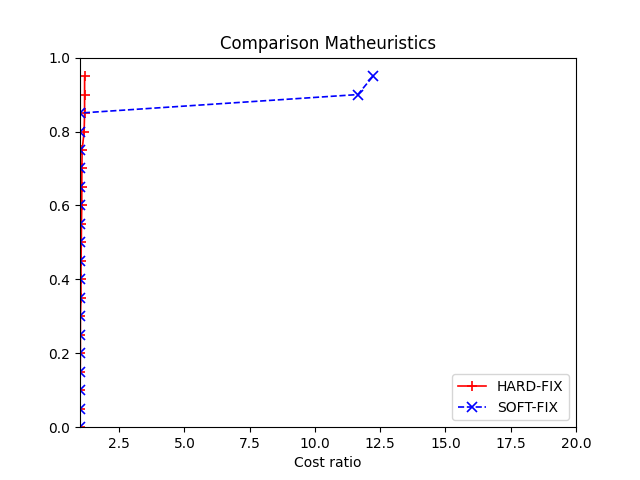
\includegraphics[width=0.6\textwidth]{images/final_math.png}
	\caption{The comparison between the Matheuristics.}
	\label{fig:result-math}
\end{figure}

It is possible to state that - except for particular instances - these two methods are providing the same performances. On the other hand, if we zoom the left side of the previous chart we can see the real difference between the algorithms.

\begin{figure}[h]
	\centering
	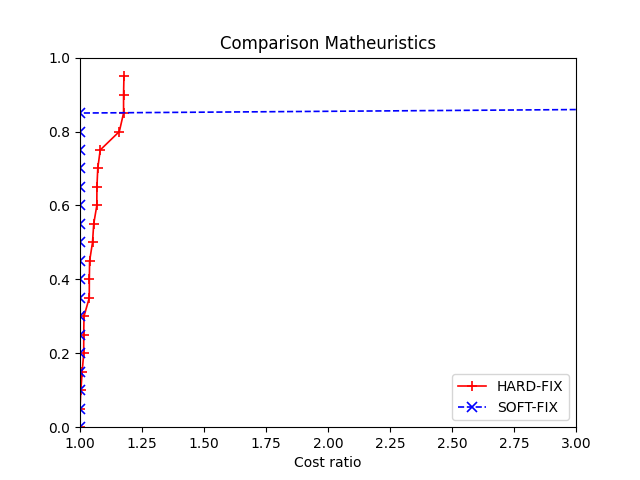
\includegraphics[width=0.6\textwidth]{images/final_math_zoom.png}
	\caption{The comparison between the Matheuristics zoomed.}
	\label{fig:result-math-zoom}
\end{figure}

In figure \ref{fig:result-math-zoom} it is indisputable that the Soft-Fixing approach, with the exclusion of the particular worse results, is the best one of this section.